\documentclass[12pt, twocolumn]{article}
\usepackage[margin=3cm]{geometry}
\usepackage{listings}
\usepackage{graphicx}
\usepackage{tikz}
\usetikzlibrary{shapes.geometric,arrows}
\renewcommand{\lstlistingname}{\textbf{Program}}
\graphicspath{Lab1}

%setting up flowcharts
\tikzstyle{startstop} = [rectangle, rounded corners, minimum width=3cm, minimum height = 1cm, text centered, draw=black, fill=red!30]

\tikzstyle{process} = [rectangle, minimum width=3cm, minimum height = 1cm, text centered, text width = 3cm, draw=black, fill=orange!30]

\tikzstyle{decision} = [diamond,  minimum width=3cm, minimum height = .5cm, text centered, text width = 3cm, draw=black, fill=green!30]

\tikzstyle{arrow} = [thick, ->,>=stealth]

\begin{document}

\begin{titlepage}
	\begin{center}
		
		
		% Upper part of the page. The '~' is needed because \\
		% only works if a paragraph has started.
		\vfill
		
		\textsc{\LARGE Experiment 2: tutor command utilization and program\\ experimentation}\\[1.5cm]
		
		\Large Adam Sumner\\[0.5cm]
		
		\Large Illinois Insititute of Technology\\[0.5cm]
		
		\Large ECE 441-01\\[0.5cm]	
		% Author and supervisor
		\noindent
		\vfill
		\large \textbf{Lab Date:} January 27th, 2015\hfill
		\large \textbf{Due Date:} February 3rd, 2015
		% Bottom of the page
		
		
	\end{center}
\end{titlepage}

\section{Introduction}
The purpose of this experiment is to acquaint the user(student) with the \textsc{tutor} monitor program along with the MC68k instruction set. The user will enter several sample programs into the \textsc{sanper-1 elu}, execute them, and debug them. 
\section{Background}
The Motorola MC68k is a CISC microprocessor that was popular during the 1980's. It has a 16-bit data bus and a 24-bit address bus. It has 8 data registers(D7-D0) for bit and bit field(1-32 bits), byte(8 bits), word(16 bits), and long-word(32 bits) operations. It also has 8 address registers (A7-A0) which can be used as software stack pointers, index registers, or base address registers. They are 32 bits wide and hold a full 32-bit address\cite{m68k}. The microprocessor has an instruction set that will not be included in this report due to its size, but several commands will be showcased that are used in the programs in this experiment. These instructions consist of at least one word, but some have as many as 11. The first word of the instruction specifies the length of the instruction, the effective addressing mode, and the operation to be performed. The remaining words, called the brief and full extension words, further specify the instruction and immediate operands. An instruction specifies the function to be performed with an OP code and defines the location of every operand. This is done through register specification, effective address, or by implicit reference. Some commonly used instructions are:
\begin{itemize}
	\item MOVE.X -\emph{Load and store. Copies an 8, 16, or 32 bit value from one memory location or register to another memory location or register}
	\item BRA -\emph{Branch. Program execution continues at location + displacement}
	\item Bcc -\emph{Branch Conditionally. If the specified condition is true, program execution continues at location + displacement}
	\item CMP.X -\emph{Compare. Subtracts the source operand from the destination data register and sets the condition codes according to the result.}
\end{itemize}
\section{Equipment/Procedure}
\subsection{Equipment}
\begin{itemize}
	\item \textsc{SANPER-1 Educational Lab Unit}
	\item Computer with TUTOR software
\end{itemize}
\subsection{Procedure}
Due to the length of each procedure, it will not be covered in depth in this report. The procedure for this experiment involved loading several pieces of code given in the experiment guide and following the instructions for each piece respectively.
\section{Results}
The software was implemented into the \textsc{sanper-1 elu} and the procedure was followed correctly. The final results of each piece of code can be found in Section \ref{appendix}.
\section{Discussion}
\subsection{Answers to Follow Up Questions}
\subsubsection{Program 1}
\begin{enumerate}
	\item A fully commented version of the original program
	\subitem \hspace{-0.7cm}\textbf{Answer:} Program is located in Section \ref{Prog1or}
	\item A fully commented version of the program written for Procedure \#9
	\subitem \hspace{-0.7cm}\textbf{Answer:} Program is located in Section \ref{Prog1}
	\item Discuss the function of each register used in the original problem.
	\subitem \hspace{-0.7cm}\textbf{Answer:} A0 and A1 are the boundary addresses. D7 is used to call the trap function and D0 holds the value \$FFFF. 
	\item Discuss the advantages of the pre-decrementing and post-incrementing addressing modes.
	\subitem \hspace{-0.7cm}\textbf{Answer:} There are no major differences/advantages to using either other than one adds and the other subtracts. In the end, they can accomplish the same thing. The key is to pick one that suits the implementation of the design
\end{enumerate}

\subsection{Program 2}
\begin{enumerate}
	\item A fully commented version of the original program
	\subitem \hspace{-0.7cm}\textbf{Answer:} Program is located in Section \ref{Prog2}
	\item List and explain the result of Procedure \#10
	\subitem \hspace{-0.7cm}\textbf{Answer:} It changed the count down from FFFF to 000F which sped up printing of the character to the terminal. 
	\item Write a subroutine that outputs any character once. The character to be outputted will be passed to this subroutine through Data Register D1.
	\subitem \hspace{-0.7cm}\textbf{Answer:} Program is located in Section \ref{Prog2sub}
	\item What is the effect of changing the instruction at address \$914 to "BRA 904"?
	\subitem \hspace{-0.7cm}\textbf{Answer:} No difference, the character will still be initialized in D0
	\item Outline the steps involved in the execution of the instructions at addresses \$90A and \$910. Discuss the usefulness of this combination of instructions.
	\subitem \hspace{-0.7cm}\textbf{Answer:} The instruction is to test the condition, decrement the data register, then branch to the specified label. In this code, it essentially acts as a timer as it branches to the same DBEQ instruction until the condition fails. It can be used to create a "hack" timer function
	\item List the major benefits of using TRAP instructions.
	\subitem \hspace{-0.7cm}\textbf{Answer:} Trap functions allow for an abstraction of very useful commonly used functionalities such as reading in data or outputting something to the terminal. It allows the programmer to easily use things like i/o without having to redefine them every single time
\end{enumerate}
\subsection{Program 3}

\begin{enumerate}
	\item A fully commented version of the original program
	\subitem \hspace{-0.7cm}\textbf{Answer:} Program is located in Section \ref{Prog3}
	\item Discuss how you would have implemented this program were TRAP Function No. 227 not available.
	\subitem \hspace{-0.7cm}\textbf{Answer:} Without Trap 227, the user would have to do it character by character. This would involve using Trap 248
	\item After executing the program, what is the final value of A5, and why?
	\subitem \hspace{-0.7cm}\textbf{Answer:} A5 points to the last byte in the output string plus one. This is because the string also includes a null byte.
\end{enumerate}

\subsection{Program 4}

\begin{enumerate}
	\item A fully commented version of the original program
	\subitem \hspace{-0.7cm}\textbf{Answer:} Program is located in Section \ref{Prog4}
	\item Draw a flowchart for the program.
	\subitem \hspace{-0.7cm}\textbf{Answer:} Flowchart is located in Section \ref{Prog4Flo}
	\item Describe the differences between the MOVE and MOVEQ instructions. Under what conditions is it advantageous to use one instruction over the other?
	\subitem \hspace{-0.7cm}\textbf{Answer:} MOVEQ is used to move immediate data while MOVE is general purpose and can move data from registers or immediate data. MOVEQ should always be used when immediate data is being loaded/stored. It is much more efficient than using the MOVE instruction. MOVE should be used when loading/storing data from a register/memory location.
	\item Discuss the usefulness of the CMPM instruction.
	\subitem \hspace{-0.7cm}\textbf{Answer:} CMPM allows for condensing multiple operations into one instruction. It lets the developer write less lines of code for efficiency.
	\item What instruction sets the Condition Code bits for the BNE instruction at address \$1018?
	\subitem \hspace{-0.7cm}\textbf{Answer:} CMPM sets the condition codes for BNE
\end{enumerate}
\subsection{Program 5}

\begin{enumerate}
		\item A fully commented version of the original program
		\subitem \hspace{-0.7cm}\textbf{Answer:} Program is located in Section \ref{Prog5}
		\item Examine the program and describe how the sorting algorithm has been implemented.
		\subitem \hspace{-0.7cm}\textbf{Answer:} It's a classic bubble sort. The program iterates through the list checking each value in the list to each other. Starting with the first value in the list, it then ``floats" up if it is less than the adjacent value in the list. This iteration continues until the list is sorted. It should be noted that this is a terrible sorting algorithm to implement with a time complexity of $\mathcal{O}(n^2)$. The best algorithm to use should be merge sort which has time complexity $\mathcal{O}(n\log n)$.
		\item Describe the significance of the SWAP instruction. Assume for a moment that the 68000 does not have a SWAP instruction. List the set of instructions, in the proper sequence that are necessary to replace the SWAP instruction.
		\subitem \hspace{-0.7cm}\textbf{Answer:} The SWAP function is what allows the values to ``float" into their correct spot in the list easily without having to use an extra data register to store temporary data and manually implement a swap algorithm. Without SWAP, use MOVE to copy temp data of first number, MOVE adjacent data into memory location of what was just saved into the register, then MOVE the data from the register into the memory location that was just moved to the location where the temporary data was taken.
		\item Describe the function and advantages of the ADDQ and SUBQ instructions.
		\subitem \hspace{-0.7cm}\textbf{Answer:} They are quick instructions designed for immediate values. They use less bus cycles to execute.
		\item Describe the differences between the ADD and ADDQ instructions.
		\subitem \hspace{-0.7cm}\textbf{Answer:} ADDQ can only handle immediate values while ADD is general purpose. ADDQ is a faster instruction.
		\item Describe the differences between the SUB and SUBQ instructions. 
		\subitem \hspace{-0.7cm}\textbf{Answer:}  SUBQ can only handle immediate values while SUB is general purpose. SUBQ is a faster instruction.
		\item Describe the sequence of events that occurs during the execution of the instruction
		located at address \$2004.
		\subitem \hspace{-0.7cm}\textbf{Answer:} The value at memory address A0 is compared to the value at memory address (A0 + word size).
\end{enumerate}
\subsection{Program 6}
\begin{enumerate}
	\item A fully commented version of both programs
	\subitem \hspace{-0.7cm}\textbf{Answer:} The original program is located in Section \ref{Prog6} and the modified version is in Section \ref{Prog68}.
	\item Draw a flowchart of the program, and discuss the insertion algorithm.
	\subitem \hspace{-0.7cm}\textbf{Answer:} The flowchart is shown in Section \ref{prog6flo}. It's an algorithm that shifts the list as it compares the values to find where an insertion is appropriate. This enables it to preserve the integrity of the list without having to overwrite data.
\end{enumerate}
\subsection{Analysis}
There is little to discuss on the results obtained, as the results obtained were merely knowledge gained by the student on how to successfully load and execute programs into the \textsc{sanper-1 elu}. However, this knowledge should carry with the student for future lab experiments as debugging and executing programs is a must have skill.
\onecolumn
\section{Conclusion} 
Overall this lab was a success. The student was successfully able to load, debug, and execute MC68k programs using the \textsc{tutor} software. From here, the student can build upon this knowledge to develop more complex programs for analysis of the machine.
\section{Appendix}
\label{appendix}
\subsection{Code}
\lstset{language=[Motorola68k]Assembler}
\subsubsection{Program 1: \normalfont Fill a Block of Memory Original}\label{Prog1or}
\lstinputlisting{2_1.X68}
\subsubsection{Program 1: \normalfont Fill a Block of Memory Modified}\label{Prog1}
\lstinputlisting{Program2_1.X68}
\subsubsection{Program 2: \normalfont Outputting a Character to the Terminal}\label{Prog2}
\lstinputlisting{2_2.X68}
\subsubsection{Program 2: \normalfont Subroutine}\label{Prog2sub}
\lstinputlisting{2_2_sub.X68}
\subsubsection{Program 3: \normalfont Outputting a String to the Terminal}\label{Prog3}
\lstinputlisting{2_3.X68}

\subsubsection{Program 4: \normalfont Pattern Match}\label{Prog4}
\lstinputlisting{2_4.X68}
\subsubsection{Program 5: \normalfont Bubble Sort}\label{Prog5}
\lstinputlisting{2_5.X68}
\subsubsection{Program 6: \normalfont Adding a Number to a Sorted List Original Code}\label{Prog6}
\lstinputlisting{2_6.X68}
\subsubsection{Program 6: \normalfont Procedure 8 Code}\label{Prog68}
\lstinputlisting{2_6_8.X68}

\subsection{Flowcharts}\label{flowchart}

\subsubsection{Program 4}\label{Prog4Flo}
\begin{center}

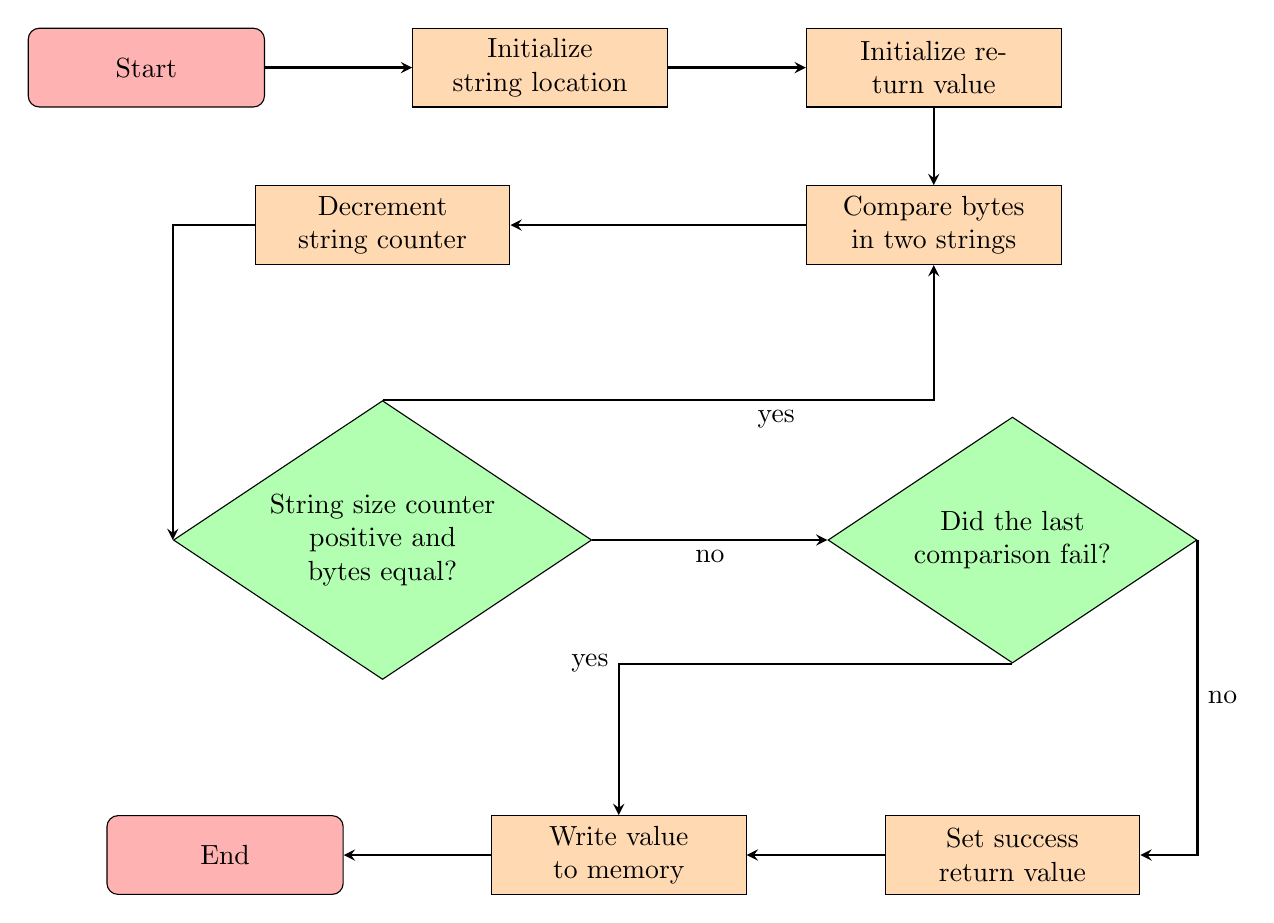
\begin{tikzpicture}[node distance = 2cm]

\node (start) [startstop] {Start};
\node (pro1)[process, right of = start, xshift = 3cm]{Initialize string location};
\node (pro2)[process, right of = pro1, xshift = 3cm]{Initialize return value};
\node (pro3)[process, below of = pro2,]{Compare bytes in two strings};
\node (pro4)[process, below of = pro1, xshift = -2cm]{Decrement string counter};
\node (dec1)[decision, below of = pro4, aspect = 1.5, yshift = -2cm]{String size counter positive and bytes equal?};
\node (dec2)[decision, right of = dec1, aspect = 1.5, xshift = 6cm]{Did the last comparison fail?};
\node (proc5)[process, below of = dec2, yshift = -2cm]{Set success return value};
\node (proc6)[process, left of = proc5, xshift = -3cm] {Write value to memory};
\node (end)[startstop, left of = proc6, xshift = -3cm]{End};


\draw [arrow] (start) -- (pro1);
\draw [arrow] (pro1)--(pro2);
\draw [arrow] (pro2)--(pro3);
\draw [arrow] (pro3)--(pro4);
\draw [arrow] (pro4.west)-|(dec1.west);
\draw [arrow] (dec1.north)-| node[anchor = north, xshift=-2cm]{yes} (pro3.south);
\draw [arrow] (dec1) -- node[anchor = north]{no} (dec2);
\draw [arrow] (dec2.south) -| node[anchor = east]{yes} (proc6.north);
\draw [arrow] (dec2.east) |- node[anchor = west, yshift=2cm]{no} (proc5);
\draw [arrow] (proc6) --(end);
\draw [arrow] (proc5)--(proc6);

\end{tikzpicture}
\end{center}
\subsubsection{Program 6}\label{prog6flo}
\begin{center}

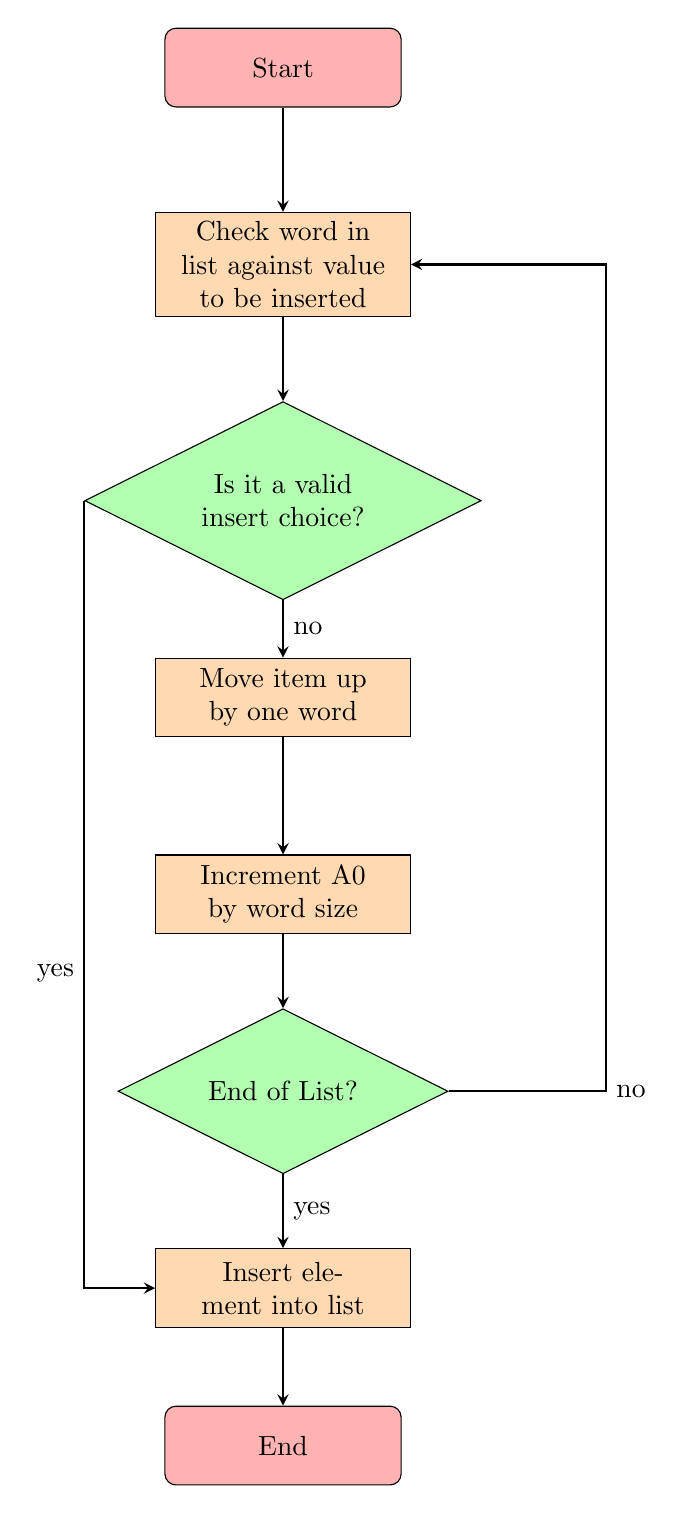
\begin{tikzpicture}[node distance = 2cm]

	\node (start) [startstop] {Start};
	\node (pro1) [process, below of =start, yshift=-0.5cm]{Check word in list against value to be inserted};
	\node (dec1) [decision, below of = pro1, aspect = 2, yshift=-1cm]{Is it a valid insert choice?};
	\node (pro2) [process, below of = dec1, yshift=-0.5cm]{Move item up by one word};
	\node (pro3) [process, below of = pro2, yshift=-0.5cm] {Increment A0 by word size};
	\node (dec2) [decision, below of = pro3, aspect = 2, yshift=-0.5cm]{End of List?};
	\node (pro4)[process, below of =dec2, yshift=-0.5cm]{Insert element into list};
	\node (end) [startstop, below of =pro4]{End};
	
	
	\draw [arrow] (start)--(pro1);
	\draw [arrow] (pro1)--(dec1);
	\draw [arrow] (dec1)--node[anchor = west]{no}(pro2);
	\draw [arrow] (dec1.west)|- node[anchor = east, yshift = 4cm]{yes}(pro4);
	\draw [arrow] (pro2)--(pro3);
	\draw [arrow]  (pro3)--(dec2);
	\draw [arrow] (dec2) -- node[anchor = west]{yes}(pro4);
	\draw [arrow] (pro4) -- (end);
	\draw [arrow] (dec2.east) -- ++(2,0) node[anchor = west, ](lowerright){no} |-(pro1.east);
	
\end{tikzpicture}
\end{center}

\begin{thebibliography}{1}
\bibitem{expman} Experiment 2 Lab Manual
\bibitem{ecbm} Educational Computer Board Manual
\bibitem{m68k}MC68K User Manual
\bibitem{sanper}SANPER-1 ELU User Manual


\end{thebibliography}

\end{document}